%%%%%%%%%%%%%%%%%%%%%%%%%%%%%%%%%%%%%%%%%%%%%%%%%%%%%%%%%
%%%%%%%%%%%%%%% author:wulemilly、msnh %%%%%%%%%%%%%%%%%%
%%%%%%%%%%%%%%%%%%%%%%%%%%%%%%%%%%%%%%%%%%%%%%%%%%%%%%%%%


\documentclass{article}
\usepackage{CJK}
\usepackage{amsmath}
\usepackage{graphicx}
\usepackage{amssymb}
\begin{CJK*}{GBK}{song}
  \title{第三章    概率论与信息论}
\begin{document}
  \maketitle
  \paragraph{}
  在这一章节,我们介绍概率论与信息论。
  \paragraph{}
  概率论是一个表示不确定性现象的数学框架。它将不确定性问题进行量化并为得到新的不确定性结论做出了公式推导。在人工智能应用领域,我们运用了概率论的两种主要方法。首先,概率法则告诉我们如何解决AI (人工智能)领域的问题,因此我们利用概率论设计相关算法来计算或运用多种表达式来近似解决该问题。其次,我们可以利用概率论和信息论从理论上来分析人工智能系统的行为。
 \paragraph{}
  概率论是科学与工程多学科交叉的一种基本工具。我们提供本章主要为致力于软件工程领域的读者提供相关的概率论知识,以确保读者可以理解本书的内容。
  \paragraph{}
  概率论为我们提供不确定性的思想并解释不确定性的原因,信息论使我们能够量化一个不确定性的概率分布。
  \paragraph{}
  如果您已经熟悉概率论与信息论,您可能希望跳过这一章,但是3.14节是我们需要关注的重点,它描述了我们用来描述机器学习的结构化概率模型的图表。如果您对这些科目没有深入的研究,本章将为您高效顺利开展深度学习项目的研究提供帮助,但是除此之外我们还是推荐您去阅读其他的相关内容	,比如Jaynes(2003)。

   %--section 1--%

  \section*{3.1 什么是概率论?}
    \paragraph{}
    计算机科学的许多分支主要是处理那些完全是确定性的实体。程序员通常可以安全地假定CPU可以完美无瑕的执行每条机器指令。在硬件中的错误确实发生,但是它还不足以在设计大多数软件应用程序的时候考虑它的影响。由于许多计算机科学家和软件工程师一般是处理比较确定性的问题,但是机器学习中大量使用概率论知识可能会令他们感到吃惊。
    \paragraph{}
    这是因为机器学习必须处理不确定的数据,有时也可能需要处理的随机数(不确定的),不确定性和随机性的产生来源于很多方面。从20 世纪80年代以来,研究人员已经为使用概率论来量化不确定性因素提供了非常可信的论据,这里提出的许多总结性的结论或启发参看Pearl (1988)。
    \paragraph{}
    许多事情都需要去推理它们存在的不确定性。事实上,除了数学可以通过定义来确定其真实性之外,很难保证任何一个绝对真实的命题,或任何一个绝对的事件都会发生。
    \paragraph{}以下是3种不确定性因素的来源:
    \subparagraph{}
    1.	在系统形成之时就存在固有的随机性。例如,在量子力学领域,亚原子的运动学都是用概率来描述的。我们也可以想象一个场景,我们假定一个动态随机的一个场景。比如一种卡牌游戏,所有的卡牌都是按照随机顺序排列的。
     \subparagraph{}
     2.	不完全的可观测性。当我们无法观测到所有的变量是如何驱动这个系统的时候,即便是个确定的系统也存在不确定性。例如一个蒙提霍尔问题。 你参加电视台的一个抽奖节目。台上有三个门,一个后边有汽车,其余后边是山羊。主持人让你任意选择其一。然后他打开其余两个门中的一个,你看到是山羊。这时,他给你机会让你可以重选,也就是你可以换选另一个剩下的门。那么,你换不换?这样的问题选手选择的结果是确定的,但是站在选手的角度来说,选择又是随机的。
     \subparagraph{}
     3.	模型的不完整性。当我们使用一个模型,这个模型里面有些我们观测到的一些信息必须舍弃的时候,那么,舍弃这些信息就会对这个模型的预测产生不确定性的影响。例如,假设我们造了一个机器人,它可以精确地观察到它周围的每一个物体的位置。当这个机器人对物体位置进行预测时,把空间离散化了,那么离散化就会给机器人带来许多不确定性因素。每个物体都可能出现在在它被观察到的离散单元内的任何位置。
    \paragraph{}
    在许多情况下,使用一个比较简单,但是不确定的规则比使用一个复杂但是确定的规则更实际。即便真是的规则是确定的,但是我们可以让我们的模型非常接近真是但是非常复杂的规则。比如一个非常简单的一个规则,我开一枪,所有的鸟都会飞这样一个模型,这个模型很好建立,也很好用。但是往深在想一下,如果那一堆鸟中,有还没有学会飞的鸟,有生病了飞不了的鸟,有受伤了飞不了的鸟等等等等…要把所有这些问题考虑进去,去建立这样一个确定的模型,这是不切实际的。
    \paragraph{}
    所以,我们需要一个表示和推理的不确定性的手段,概率论可以为我们提供一些我们想用在人工智能上的一些工具,但是可能它给我们呈现出的结果并不是立马就能观测到的。概率论的出现本来是用于分析事件的频率。很容易可以概率论是如何使用的,比如去描述在一个扑克游戏中的某一手牌。这些事件通常是可重复的。假设某个事件发生的概率为p,当我们重复这个事件的时候,他的结果发生的概率始终是p。这种推理似乎并不适用于不可重复的命题。如果一个医生分析一个病人,并说,病人有40\%的机会患流感,我们不可能说是拥有无限个这样的病人也没有任何理由相信同样的病人会得同样的病。但有不同的基本条件。在医生诊断病人的时候,我们使用概率来表示一件事情的可信度,用1 表示这个病人一定会得流感,用0表示这个病人一定不会得流感。前一种概率,直接关系到事件发生的概率,被称为古典概型。而后者,与确定性的定性水平有关,被称为贝叶斯概率。
    \paragraph{}
    如果我们希望常识性的东西具有不确定性,那么唯一的方法就是,使用贝叶斯概率来当成我们所熟知的古典概型。例如,当我们知道一个玩家手上的牌之后,去计算他能赢的概率的时候,我们会使用和计算某个具有确定症状的病人去计算他的犯病概率的一样的公式。关于为什么一小部分常识性的假设意味着两种概率类型必须受到同一公理约束的更多细节性问题可以参看(Ramsey(1926))。
    \paragraph{}
    概率可以看作是一种处理不确定性逻辑的扩展,逻辑提供了一套正式的规则用于确定什么样的命题是隐含的真或假的假设,概率论提供了一套正式的规则,用于确定一个命题为真的可能性及命题的其他可能性。

    %--section 2--%

    \section*{3.2 随机变量}
    \paragraph{}
    一个随机变量是一个可以随机抽取不同的值的变量。我们通常以大写字母如$X,Y,Z,W…$表示随机变量,而以小写字母如$x,y,z,w…$表示实数。例如,$x_1$ 和$x_2$都是随机变量X 的取值。对于随机向量,我们用X表示随机变量和用x表示该随机变量的一个值。对其本身而言,一个随机变量只是描述一种状态的可能性,它必须加上一个概率分布,指定每个状态的可能性大小。
    \paragraph{}
    随机变量可以是离散的或连续的。离散型随机变量是一个具有有限个或可列无限多个状态。需要注意的是,这些状态不一定是整数,它们也可以只是被命名为不考虑有任何数值的状态。一个连续的随机变量与一个真实值相关。

    %--section 3--%

   \section*{3.3 概率分布}
    \paragraph{}
    概率分布是描述一个随机变量的可能性或一个随机变量集合中每一个变量可能的状态。我们描述的概率分布的方式取决于变量是离散的或连续的。
    \subsection*{3.3.1 离散变量及概率质量函数}
    \paragraph{}
    离散变量的概率分布可以用概率质量函数描述(PMF)。我们通常表示概率质量函数用大写字母P。 通常我们将每个随机变量对应不同的概率质量函数,读者必须推断出的哪一个概率质量函数对应该随机变量的结果,而不是通过函数的名字判断;$P(\mathrm{x})$ 和$P(\mathrm{y})$通常是不相同的。
    \paragraph{}
    概率质量函数映射是指随机变量的一个状态到随机变量在该状态下的概率。概率$\mathrm{x} = x$被记为$P(x)$,当概率为1时表明$\mathrm{x} = x$是必然的,当概率为0 时表明$\mathrm{x}=x$是不可能的,有时为了更好的理解概率质量函数,我们可以明确的表示随机变量的名称:$P(\mathrm{x} = x)$。 有时,我们先定义一个变量,然后使用$\sim$符号指定其分布如下:$\mathrm{x}\sim{P(x)}$。
    \paragraph{}
    概率质量函数可以同时作用于多个变量。这种具有多个变量的概率分布被称为联合概率分布。$P(\mathrm{x} = x, \mathrm{y} = y)$同时表示概率$\mathrm{x} = x$ 和$\mathrm{y} = y$。我们还可以简写为$P(x, y)$。
    \paragraph{}
    为了计算一个随机变量x的概率质量函数,函数P必须满足下列性质:
    \subparagraph{}
     1.$P$的取值必须是x的所有可能状态的集合。
    \subparagraph{}
     $2.\forall\mathrm{x} \epsilon x,0 \leq P(x) \leq 1.$ 一个不可能事件的概率为0,没有任何一种状态比0还小。同样,确定发生的事件的概率为1,没有任何一种状态比1还大。
    \subparagraph{}
     $3.\sum _{\mathrm{x} \epsilon x} P(x) = 1.$我们将此属性称为归一化。如果没有这个属性,通过计算许多事件发生的概率我们可能获得一个大于1 概率。
    \paragraph{}
    例如,考虑一个单一的离散随机变量x 有k种不同的状态。我们可以通过计算它的概率密度函数得到x 是均匀分布的(也就是说,每一种状态的可能性相等)。

    \begin{equation}
    P(\mathrm{x}=x_i )=\frac{1}{k} \tag{3.1}
    \end{equation}
    \paragraph{}

    对于所有的i,我们可以看出这符合概率质量函数的要求。因为k 是一个正整数,所以值$\frac{1}{k} $是正的。我们也看出
    \begin{equation}
    \sum_i P(\mathrm{x}=x_i )=\sum_i\frac{1}{k}=\frac{k}{k}=1 \tag{3.2}
    \end{equation}
    \paragraph{}
    因此,概率分布是适当的归一化。
    \subsection*{3.3.2 连续变量及概率密度函数}
    \paragraph{}
    当计算连续型随机变量的概率分布时,我们使用概率密度函数(PDF)而不是概率质量函数。要成为一个概率密度函数,函数P必须满足下列性质:
    \subparagraph{}
     1.$P$的取值必须是x的所有可能状态的集合。
    \subparagraph{}
     $2.\forall \mathrm{x} \epsilon x,P(x)\geq0.$ 需要注意的是,我们不要求$p(x) \leq 1$。
    \subparagraph{}
     $3.\int p(x)dx = 1$ 。
    \paragraph{}
    一个概率密度函数不给它特定的概率,而是落在一个无穷小的区域的概率,可以近似的表示为$p(x)\delta x$。
    \paragraph{}
    我们通过整合密度函数来找到点集的实际概率。具体而言,x 位于某一集合S的概率是由$P(x)$在该集合上的积分得到的。举一个单变量的例子,x在区间[a,b]的概率是通过$\int_{[a,b]}p(x)dx$得到的。
    \paragraph{}
    举一个例子,概率密度函数相当于一个连续随机变量考虑实数区间上的均匀分布的一个特定的概率密度。我们可以用一个函数$u(x;a,b)$表示,其中a和b是区间的两个端点,且$b> a$。符号“;”表示参数化;我们认为x是函数的参数,而a和b 是定义函数的参数。为了确保概率密度都在区间范围内,我们可以说对于所有的$x\not\in[a,b]$,其$u(x;a,b)=0$。在[a,b]区间内的$u(x;a,b)=\frac{1}{(b-a)}$。我们可以看到结果是非负的,其值最大为1。我们经常将$x$在区间[a,b]的概率分布表示为$x \sim U(a, b)$。

    %--section 4--%

    \section*{3.4 边缘概率}
    \paragraph{}
    有时我们知道一组变量的边缘概率,同时也想得到子变量的概率分布。我们把子变量的概率分布叫做边缘概率分布。
    \paragraph{}
    例如,假设我们有离散随机变量x和y,我们知道P(x,y),则可以计算P(x)为:
    \begin{equation}
     \forall x \epsilon X,P(x=\textbf{X})=\Sigma_yP(x=X,y=Y)  \tag{3.3}
    \end{equation}
    “边缘概率”的名字来源于边缘概率的计算过程。当P(x,y)的值以x为行,y为列写在表格中,将行的数值求即为P(x)的值。
    \paragraph{}
    对于连续型变量,我们需要积分而不是求和:
    \begin{equation}
      p(x)=\int p(x,y)dy  \tag{3.4}
    \end{equation}

    %--section 5--%

     \section*{3.5 条件概率}
    \paragraph{}
    很多情况下,我们更感兴趣的是考虑事件A已经发生的条件下事件B的概率,这就叫条件概率。我们可以将$\mathrm{x}=x$在$\mathrm{y}=y$ 的条件下的概率表示为$P(\mathrm{y} = y | \mathrm{x} = x)$。该条件概率可以用公式计算:
    \begin{equation}
      P(\mathrm{y} = y | \mathrm{x} = x)=\frac{P(\mathrm{y} = y | \mathrm{x} = x)}{P( \mathrm{x} = x)} \tag{3.5}
    \end{equation}
    \paragraph{}
    条件概率只有当$P(\mathrm{x} = x)> 0$时才能定义。我们不能计算一个从未发生过的事件的条件概率。
    \paragraph{}
    重要的是不要将条件概率与通过采取一定措施计算将会发生事情的概率混淆,条件概率可以形象的解释为一个德国人的德语说的相当好,但如果一个随机选择的人教他学德语,但他们的原国籍不会改变。计算一个动作的因果被称为做干预查询。干预查询是因果模型的领域,我们不在这本书中探索。


    %--section 6--%

 \section*{3.6 条件概率链式法则}
    \paragraph{}
    在许多随机变量的联合概率分布可以分解为一个变量的条件分布:
    \begin{equation}
      P(x^{(1)},\cdots,x^{(n)})=P(x^{(1)})\prod^{n}_{i=2} P(x^{(i)}|x^{(1)},\cdots,x^{(i-1)}) \tag{3.6}
    \end{equation}
    \paragraph{}
    这就叫做链式法则或乘积法则,可由公式(3.5)中的条件概率的定义来推导。例如,将其定义两次我们可以得到:
    $$ P (a, b, c) = P (a | b, c)P (b, c)$$
    $$ P (b, c) = P (b | c)P (c)$$
    $$ P (a, b, c) = P (a | b, c)P (b | c)P (c)$$

    %--section 7--%

    \section*{3.7 独立性和条件独立性}
    \paragraph{}
    两个随机变量x和y是独立的,他们的概率分布可以表示为一个事件的两个因素,一个只与x相关,另一个只与y相关:
    \begin{equation}
      \forall \mathrm{x}\epsilon x,\mathrm{y}\epsilon y,p( \mathrm{x} = x,\mathrm{y} = y )=p( \mathrm{x} = x)p(\mathrm{y} = y )\tag{3.7}
    \end{equation}
    \paragraph{}
    两个随机变量x和y是相互独立的,若有一个随机变量z,在变量z的条件下x和y的条件概率分布为:
    \begin{equation}
    \forall \mathrm{x}\epsilon x,\mathrm{y}\epsilon y,\mathrm{z}\epsilon z,p( \mathrm{x}=x,\mathrm{y}=y|\mathrm{z}=z )=p( \mathrm{x}=x|\mathrm{z}=z)p(\mathrm{y}=y|\mathrm{z}=z ) \tag{3.8}
    \end{equation}
    \paragraph{}
    我们可以用更简便的方式表达独立性与条件独立性:$x\bot y $意味着x和y是相互独立的,而$x\bot y | z$则表示x和y 在z的条件下是相互独立的。

    %--section 8--%

     \section*{3.8 期望,方差和协方差}
    \paragraph{}
    函数$f(x)$的期望或期望值是x与其相对应的概率分布$P(x)$的乘积的平均值。对于离散型变量可以做一个求和的计算:
    \begin{equation}
     E_{x\sim P}[f(x)]=\sum _x P(x)f(x)  \tag{3.9}
    \end{equation}
    \paragraph{}
    对于连续型变量,它是用一个积分计算的:
    \begin{equation}
       E_{x\sim P}[f(x)]=\int P(x)f(x)dx   \tag{3.10}
    \end{equation}
    \paragraph{}
    当需要计算某一个变量时,我们可以在计算期望用其变量名作为下标,例如$E_x[f(x)]$。在所求的随机变量确定的情况下,也可以不用变量名作为下标,可将其省略,如$E[f(x)]$。 默认情况下,可以用$E[?]$表示所有括号内的随机变量的平均值。同样地,当没有歧义时,我们可以省略方括号。
    \paragraph{}
    期望是线性的,例如:
    \begin{equation}
      E_x [\alpha f(x)+\beta g(x)]=\alpha E_x[f(x)]+\beta E_x[g(x)]  \tag{3.11}
    \end{equation}
    \paragraph{}
    $\alpha$和$\beta$不依赖与$x$。
    \paragraph{}
    方差就是随机变量x的函数的数学期望,表达式如下:
    \begin{equation}
      Var(f(x))=E[(f(x)-E[f(x)])^2] \tag{3.12}
    \end{equation}
    \paragraph{}
    当方差很小时,$F(x)$的值接近他们的期望值。方差的平方根被称为标准偏差。
    \paragraph{}
    协方差表示两个变量之间的线性关系,以及变量之间的线性程度:
    \begin{equation}
      Cov(f(x),g(y))=E[(f(x)-E[f(x)])(g(y)-E[g(y)])] \tag{3.13}
    \end{equation}
    \paragraph{}
    协方差的绝对值较大意味着两个变量总体误差的期望越大。如果协方差的值是正值,说明其中一个变量大于自身的期望值时另外一个变量也大于自身的期望值;如果协方差的值是负值,说明其中一个变量大于自身的期望值的同时另外一个却小于自身的期望值,反之亦然。其他测量方法如相关系数,用来表示两个变量之间线性关系的紧密程度,而不单单是一个独立变量的受影响程度。
    \paragraph{}
    协方差和相关是有联系的,但实际上是不同的概念。两个变量的协方差为0表示不相关,两个变量的协方差不为0则表示相关。然而,协方差的独立性具有不同的属性,对于两个变量,如果协方差为0,则表示它们之间一定没有线性关系。独立性比协方差的要求更严格,因为独立性也不包括非线性关系,也就是说两个变量之间有关系,但是它的协方差为0。例如,假设我们的第一个样本的一个实数$x$在区间[-1,1]之间均匀分布,下一个样本是一个随机变量s。当概率为1/2,$s$的值为1。否则,$s$的值为-1。我们生成一个随机变量$y$且$y=sx$。 显然,$x$和$y$是不独立的,因为x完全决定了y的大小,但是$ Cov(x, y) = 0$。
    \paragraph{}
    一个随机向量$x\in R_{n}$的协方差矩阵是一个n×n矩阵,这样:
    \begin{equation}
      Cov(x)_{i,j}= Cov(x_i,x_j) \tag{3.14}
    \end{equation}
    \paragraph{}
    协方差的对角线元素给出方差:
    \begin{equation}
       Cov(x_i,x_j)=Var(x_i) \tag{3.15}
    \end{equation}

    %--section 9--%

    \section*{3.9 常用概率分布}
    \paragraph{}
    这里介绍几种在机器学习领域比较常用的概率分布。
    \subsection*{3.9.1 伯努利分布}
    \paragraph{}
    伯努利分布是一种是离散型的随机变量,变量只能取两个值,非0即1。它用一个参数 ,来衡量这个随机变量等于1的可能性。它有以下几项特征:
    \begin{equation}
     P(X=1)=\phi   \tag{3.16}
    \end{equation}
    \begin{equation}
     P(X=0)=1-\phi   \tag{3.17}
    \end{equation}
    概率公式
    \begin{equation}
     P(X=x)=\phi^{x} (1-\phi)^{1-x}  \tag{3.18}
    \end{equation}
    数学期望
    \begin{equation}
     E_{x}(X)=\phi  \tag{3.19}
    \end{equation}
    方差
    \begin{equation}
     Var_{x}(X)=\phi(1-\phi)  \tag{3.20}
    \end{equation}
    \subsection*{3.9.2 多项分布}
    \paragraph{}
    多项分布是一种是离散型的随机变量,变量取$k,k$为有限个数。它通过一个向量$ p_{i}\in [0,1]^{k-1} $ 来描述, 说明$ p_{i} $ 了第i次此事件发生的可能性。最终为$k$。多项分布是通常用于事件发生的情况不止一种的状况下。因此,我们通常不认为状态1和数值1等价,等等。所以,我们通常不需要计算多项分布的期望值和方差。
    \paragraph{}
    伯努利分布和多项分布足以描述他们的领域的任何分布。因为离散模型使用枚举方法列出所有的状态,是可行的。然而当处理连续型变量时,就会出现不可数的情况出现。所以少量参数的分布必须严格限制在这两种分布内。
    \subsection*{3.9.3 正太(高斯)分布}
    \paragraph{}
    最常用的用于描述实数的分布规律的分布为正态分布,也被称为高斯分布:
    \begin{equation}
      N(x,\mu,\sigma^{2})=\sqrt{\frac{1}{2\pi\sigma^{2}}}\mathrm{exp}(-\frac{1}{2\pi\sigma^{2}}(x-\mu)^{2})  \tag{3.21}
    \end{equation}
   \begin{figure}[!htb]
    \centering
   \centerline{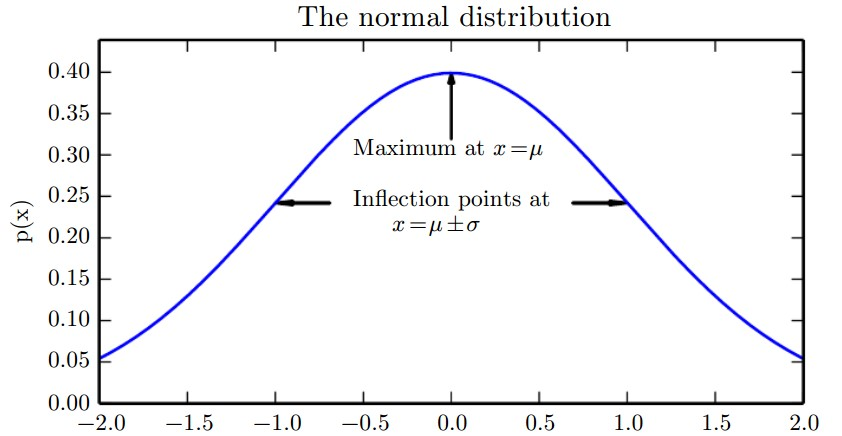
\includegraphics[width=3.5in]{fig/chap3/3_1.jpg}}
   \label*{图:3.1}
   \end{figure}
   \paragraph{}
    图3.1为正太分布密度函数的一个描述。正态分布是典型的钟形曲线,$\mu$为x轴的中间峰值。宽度由$\sigma$控制。此图中的例子,是一个$\mu$ 为0,$\sigma$为1的正太分布。
    \paragraph{}
    正太分布用两个参数$\mu\in \mathrm{R}$和$ \sigma\in (0,\infty)$ 来描述。参数μ 为中心峰值坐标。同样它的方差$E(\mathrm{x})= \mu$,用$\sigma$表示标准差, $\sigma^{2}$表示方差。
    \paragraph{}
    当我们计算概率密度函数的时候,我们需要对$\sigma$进行平方和取倒数。当我们需要频繁的使用不同的参数去计算概率密度函数的时候,我们可以引入一个参数$\beta\in (0,\infty)$ 控制正太分布的精度和逆方差来更有效的参数化正太分布。
   \begin{equation}
      N(x,\mu,\beta^{-1})=\sqrt{\frac{\beta}{2\pi}}\mathrm{exp}(-\frac{\beta}{2\pi}(x-\mu)^{2})  \tag{3.22}
    \end{equation}
    \paragraph{}
    许多情况下使用正太分布是一种分成明智的选择。在没有先验知识的情况下,采用正太分布是非常好的选择有以下两个原因:
    \subparagraph{}
    第一,我们希望模型的许多分布能真正接近正常分布。中心极限定理表明,许多独立的随机变量的总和是近似正态分布的。这就意味着在实际实践中,许多复杂的系统可以成功地建模为正态分布,即使该系统可以被更结构化的去分解。
    \subparagraph{}
    第二,可能的大部分概率分布具有相同的方差,而正态分布对实数的最大不确定度进行编码。因此,我们可以认为正态分布是一个最少将先验知识插入到模型中的一种分布。充分开发和证明这个想法需要更多的数学工具。此部分见章节19.4.2。
    \paragraph{}
    正太分布推广到$\mathrm{R}^{n}$,在这种情况下,它被称为多元正态分布。可以被一个正定对称矩阵$\sum$进行参数化。
    \begin{equation}
      N(x,\mu,\sum)=\sqrt{\frac{1}{2\pi^{n}\mathrm{det}(\sum)}}\mathrm{exp}(-\frac{1}{2}(x-\mu)^{T}\sum^{-1}(x-\mu))  \tag{3.23}
    \end{equation}
    \paragraph{}
    此处的$\mu$的意思和前面的是一样的,只不过现在是个向量。参数$\sum$给出了次分布的协方差矩阵。对于单因素情况下,当我们希望去计算不同参数值的概率密度函数的时候,协方差是不是一个有效的方式计算的参数化的分布。因此我们需要对$\sum$进行转置去评估概率密度函数。我们可以用一个精度矩阵$\beta$来替换。
    \begin{equation}
      N(x,\mu,\beta^{-1})=\sqrt{\frac{\mathrm{det}(\beta)}{2\pi}}\mathrm{exp}(-\frac{\beta}{2\pi}(x-\mu)^{T}(x-\mu))  \tag{3.24}
    \end{equation}
    \paragraph{}
    我们经常将协方差矩阵修正伪对角矩阵。更简单的一个例子,各向同性的高斯分布,其协方差矩阵是系数位常数的单位矩阵。
    \subsection*{3.9.4 指数分布和拉普拉斯分布}
    \paragraph{}
    在深度学习中,我们经常希望在x = 0的有一个尖锐点的概率分布。要做到这一点,我们可以使用指数分布:
    \begin{equation}
      p(x;\lambda)=\lambda1_{x\geq0}\mathrm{exp}(-\lambda x)  \tag{3.25}
    \end{equation}
    \paragraph{}
    指数分布采用函数$1_{x\geq0}$ 表示分配概率为零的X的所有负值.而拉普拉斯分布则是可以让概率在点$\mu$处取得峰值。
    \begin{equation}
     \mathrm{Laplace}(x;\mu;\gamma)=\frac{1}{2\gamma} \mathrm{exp}(-\frac{|x-\mu|}{\gamma}) \tag{3.26}
    \end{equation}
    \subsection*{3.9.5 狄拉克分布和经验分布}
    \paragraph{}
    在某些情况下,我们希望指定的概率分布在围绕某个点的集群中。那么呢,我们可以通过定义一个狄拉克$\delta$函数实现。
    \begin{equation}
      p(x)=\delta(x-\mu)  \tag{3.27}
    \end{equation}
    \paragraph{}
    狄拉克$\delta$函数定义为在除了零以外的点函数值都等于零,而其在整个定义域上的积分等于1。狄拉克$\delta$函数不像一个普通的函数,一个输入得到一个真正的输出。相反狄拉克$\delta$函数它是一种不同类型的数学对象,称为广义函数,他是根据属性的集成定义的。我们可以认为狄拉克$\delta$函数的目的就是把除$\mu$点以外的值都无限接近于0。
    \paragraph{}
    通过定义$P(x)$是$\delta$函数平移$-\mu$所得到的无限窄的一个函数,在$x=\mu$ 时值取无限大。狄拉克分布是经验分布的一部分,把概率的$1/m$分布在每个$m$点$x^{(1)}...x^{(m)}$上形成一个给定的数据集或样本集合。
    \begin{equation}
     \hat{p}(x)=\frac{1}{m}\sum_{i=1}^{m}\delta(x-x^{(i)}) \tag{3.28}
    \end{equation}
    \paragraph{}
    在经验分布的连续型变量中使用狄拉克分布是有必要的,但是在离散型变量中,情况就简单许多。在离散型变量中,可以慨括为多项分布,与每个可能的输入值相关联的概率,简单地等于在训练集的该值的经验频率。我们可以把从训练样本数据集形成的经验分布看做成是对我们指定数据模型的训练。另外一种可以最大限度的提高训练数据的概率的可能性的经验分布参见5.5小节。
    \subsection*{3.9.6 混合分布}
    \paragraph{}
    结合其他简单分布去定义一种新的分布是挺常见的。组合分布的一个常见的方法是构造一个混合分布。混合分布是由几项分布组成的。在每个试验中,选择哪种成分的分布产生的样本,是从多项分布中抽样单位分量所决定的。
    \begin{equation}
      p(\mathrm{x})=\sum_{i}P(c=i)P(\mathrm{x}|c=i)  \tag{3.29}
    \end{equation}
    其中$P(c)$是对成员的多项分布。
    \paragraph{}
    在前面我们已经接触到了混合分布的一个例子。经验分布的实数部分就是使用狄拉克的一个混合分布。
    \paragraph{}
    混合模型是一种用来创建一个更复杂分布的简单策略之一。在16 章我们会更加详细的去介绍简单分布到混合分布的创建。混合模型使我们能分析出一个非常重要的概念,潜在变量。潜在变量是用在我们无法观测的一种随机变量。从混合分布的单位变量$c$就可以看出。潜在变量可以通过联合分布与$x$相关。在这种情况下,$P(\mathrm{x},c)=P(\mathrm{x}|c)P(c)$.其中$P(c)$是基于潜在变量的,而$P(\mathrm{x}|c)$ 可以根据可见变量和潜在变量去决定$P(\mathrm{x})$的形状,虽然没有参考隐藏变量,但是也能描述$P(\mathrm{x})$。
    \paragraph{}
    非常重要和常用的联合模型是高斯混合模型,其中$p(\mathrm{x}|c=i)$是高斯的。每个组成部分都有在自己单独的均值$\mu^{(i)}$和方差$\ sum^{(i)}$. 有些混合模型可能有更多的约束。例如:协方差可以通过约束$\sum^{(i)}=\sum\forall i$来共享成员。作为一个单一的高斯分布, 混合高斯模型可以为每个组件是对角或各向同性的协方差矩阵的约束。
    \paragraph{}
    除了均值和方差,高斯混合分布指定了每个$i$的先验分布$\alpha_{i}=P(c=i)$。先验是指已经知道$c$的情况下观察到$x$。 做一下对比,$P(c|x)$是一个后验概率,因为它在观察到$x$ 后才计算。高斯混合模型是常用的近似密度,因为任何平滑的密度都可以被多变量高斯混合模型近似。
    \begin{figure}[!htb]
    \centering
   \centerline{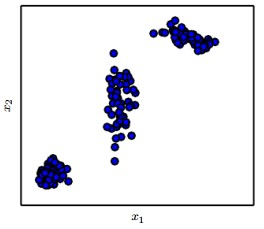
\includegraphics[width=3.0in]{fig/chap3/3_2.jpg}}
   \label*{图:3.2}
   \end{figure}
   \paragraph{}
   图3.2是高斯混合模型的样本。在这个例子中,有三个部分,从左到右,第一部分有一个各向同性的协方差矩阵,这意味着在每个方向上具有相同的方差。第二部分有一个对角协方差矩阵,这意味着它可以分别控制沿各轴方向的方差。从这个例子可以看出沿$X_{2}$轴的方差比$X_{1}$轴要大。第三部分有一个满秩的协方差矩阵,它能够单独控制任意方向上的方差。

    %--section 10--%

    \section*{3.10 常用函数的有用性质}
    \paragraph{}
    概率分布在很多函数的计算中应用广泛,特别是在深度学习模型中使用的概率分布。
    \paragraph{}
    这些函数之一就是描述S型曲线的logistic模型:
    \begin{equation}
    \sigma(x)=\frac{1}{1+\mathrm{exp}(-x)}   \tag{3.30}
    \end{equation}
    \paragraph{}
    S型曲线的logistic模型通常用于产生一个伯努利分布的参数$\varphi$,$\varphi$值的有效区间在(0,1)之间。图3.3是描述S型函数的图表,S型函数的参数过大或过小,都意味着函数变得平滑,且对其输入的微小变化不敏感。
    \paragraph{}
    另一个常见的函数是softplus 函数,参看(Dugas et al.,2001):
    \begin{equation}
    \zeta(x)=log(1+\mathrm{exp}(x))   \tag{3.31}
    \end{equation}
    \paragraph{}
    softplus 函数可以计算出正态分布的$\beta$和$\sigma$参数,其范围在$(0,\infty)$之间。当涉及S型曲线时常用该表达式。softplus 函数的名字来自于一个平滑的或"软化"版的如图3.4所示的softplus 函数的图表。
    \begin{figure}[!htb]
    \centering
   \centerline{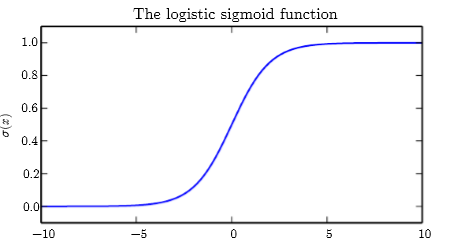
\includegraphics[width=3.5in]{fig/chap3/3_3.png}}
   \label*{图:3.3}
   \end{figure}
    \begin{figure}[!htb]
    \centering
   \centerline{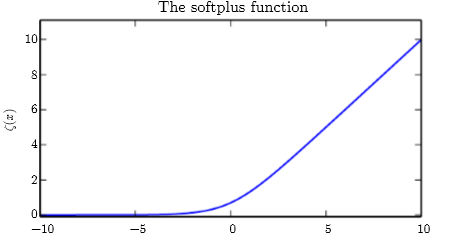
\includegraphics[width=3.5in]{fig/chap3/3_4.png}}
   \label*{图:3.4}
   \end{figure}
   \paragraph{}
   该函数具有以下性质:
   \begin{equation}
    \sigma(x)=\frac{\mathrm{exp}(x)}{\mathrm{exp}(x)+\mathrm{exp}(0)}   \tag{3.33}
   \end{equation}
   \begin{equation}
    \frac{d}{dx}\sigma(x)=\sigma(x)(1-\sigma(x))   \tag{3.34}
   \end{equation}
   \begin{equation}
    1-\sigma(x)=\sigma(-x)   \tag{3.35}
   \end{equation}
   \begin{equation}
    log\sigma(x)=-\zeta(-x)   \tag{3.36}
   \end{equation}
    \begin{equation}
    \frac{d}{dx}\zeta(x)=\sigma(x)  \tag{3.37}
   \end{equation}
   \begin{equation}
   \forall x\in(0,1),\sigma^{-1}(x)=log(\frac{x}{1-x})  \tag{3.38}
   \end{equation}
   \begin{equation}
   \forall x>0,\zeta^{-1}(x)=log(\mathrm{exp}(x)-1)  \tag{3.39}
   \end{equation}
   \begin{equation}
   \zeta(x)=\int_{-\infty}^{x}\sigma(y)dy  \tag{3.40}
   \end{equation}
   \begin{equation}
   \zeta(x)-\zeta(-x)=x \tag{3.41}
   \end{equation}
   \paragraph{}
   函数$\sigma^{-1}(x)$被称为统计的Logit模型,但是该术语很少用在机器学习中。
   \paragraph{}
   公式3.41对"softplus"给出了新的解释。Softplus函数是一个正部函数的光滑版本,$x^{+} =max{0, x}$。正部函数是负部函数的对应,$x^{-} = max{0,-x}$。为了获得一个平滑的函数,类似负部函数可以使用$\zeta(-x)$。$x$可以通过正部函数和负部函数通过$x^{+}- x^{-} = x$ 来抵消,也可以利用$\zeta(x)$和$\zeta(-x)$之间的关系来抵消,如公式3.41。

    %--section 11--%

    \section*{3.11 贝叶斯法则}
    \paragraph{}
    通常我们知道$P(y | x)$的情况下想计算$P(x | y)$,这时,如果我们还知道$P(x)$,我们就可以通过贝叶斯法则得到结果:
    \begin{equation}
   P(x|y)=\frac{P(x)P(y|x)}{P(y)} \tag{3.42}
   \end{equation}
   \paragraph{}
   需要注意的是,当公式中出现$P (y)$时,通常可以用$P(y)=\sum_{x}P (y|x)P(x)$计算,因此我们不需要去了解$P(y)$。贝叶斯规则是直接从条件概率的定义中得出的,但是我们熟悉这个名字是因为许多文本中提及才知道的。Reverend Thomas Bayes在公式中发现了一个特殊的现象,因此将其命名为贝叶斯。这里所提到的贝叶斯公式是由Pierre-Simon Laplace发现的。

    %--section 12--%

    \section*{3.12 连续变量的技术细节}
   \paragraph{}
  以恰当的形式理解连续随机变量和概率密度函数需要概率论的一个被称为测量理论数学分支的发展。测量理论是超出了这本教科书的范围,但我们可以简要的勾勒出一些测量理论的问题来解决。
   \paragraph{}
   在3.3.2节,我们看到,一个连续向量值$x$在集合$S$的概率是$P(x)$的积分。而一些集合$S$的选择可能会产生矛盾。例如,它可以构建两个集合$S1$和$S2$,即$P(x\in S1)+ P(x\in S2)> 1$但$S1 \cap S2 = \phi$.。这些集合通常是由大量使用的实数的无限精度的构造,例如分形集合或将有理数集合定义的集合。测量理论的一个重要贡献是提供一个表征的集合,我们可以计算出没有遇到矛盾的概率。在这本书中,我们只集成了相对简单的描述,所以这方面的测量理论不需要特别关注。
   \paragraph{}
   对于我们而言,测量理论在描述定理方面是非常有用的,其应用于$R_{n}$最点但不适用于一些边缘事件。测度理论提供了一个严格的方式来描述一个点集小到可以忽略不计。这个点集被称为“测量零”,我们在这本书中没有正式定义这个概念。然而,对它的理解是非常有用的,一组测量零点在我们测量的空间中没有体积,例如,当填充的多边形有正测量时,在$R_{2}$的线上有一个测量零点。同样,一个单独的点有测量零点。任何一个可数集合,每个都会有测量零点(因此所有的有理数集有测量零点)。
   \paragraph{}
   测量理论的另一个有用的术语是“几乎无处不在”,也就是除了集合的测量零点,几乎拥有其他所有的空间的属性。因为异常占据了可以忽略的空间,所以它们可以被安全地忽略许多应用程序。概率论中的一些重要结果持有所有的离散值,但只持有“几乎无处不在”的连续值。
   \paragraph{}
   连续变量的另一个技术细节是处理连续的随机变量,这是一个相互确定的函数。假设我们有两个随机变量$x$和$y$,使得$y = g (x)$,其中$g$是一个可逆的、连续的、可微变换。人们可能会想到$p_{y}(y)=p_{x}(g^{-1}(y))$.其实不是这样的。
   \paragraph{}
   举一个简单的例子,假设我们有一个随机变量$x$和$y$,均为标量,假设$y = x /2,x \in U(0,1)$。如果我们使用规则的$p_{y}(y)=p_{x}(2y)$,除了区间[0,1/2],$P_{y}$为0,在这个区间为1。这意味着下式违反了概率分布的定义。
   \begin{equation}
     \int p_{y}(y)dy=\frac{1}{2}.\tag{3.43}
   \end{equation}
   \paragraph{}
   这种常见的错误是因为它没有考虑函数$g$所引入的空间的变形。回忆一下$x$在一个体积无穷小的区域$\sigma x$的概率是$p(x)\sigma x$。由于$g$可以扩大或收缩空间,$x$空间中的无穷小体积在$y$空间中可能有不同的体积。
   \paragraph{}
   如何纠正这个问题,我们返回标量的情况下。我们需要保证其属性:
   \begin{equation}
      |p_{y}(g(x))dy|=|p_{x}(x)dx|.\tag{3.44}
   \end{equation}
   \paragraph{}
   从这一点上解决,可以得到:
    \begin{equation}
      p_{y}(y)=p_{x}(g^{-1}(y))|\frac{\partial{(x)}}{\partial(y)}|.\tag{3.45}
   \end{equation}
   \paragraph{}
   也可以用:
    \begin{equation}
      p_{x}(x)=p_{y}(g(x))|\frac{\partial{g(x)}}{\partial(x)}|.\tag{3.46}
   \end{equation}
   \paragraph{}
   在更高的维度,衍生出雅可比矩阵的行列式—矩阵的每个元素为$J_{i,j}=\frac{\partial{x_{i}}}{\partial(y_{j})}$.因此,对于实数向量$x$和$y$,
   \begin{equation}
      p_{x}(x)=p_{y}(g(x))|\det{(\frac{\partial{g(x)}}{\partial(x)})}|.\tag{3.47}
   \end{equation}

    %--section 13--%

    \section*{3.13 信息论}
   \paragraph{}
  信息理论是应用数学的一个分支,涉及如何量化信号中存在多少信息的问题。它最初被发明研究的是离散的字母在嘈杂的通道发送信息,如通过无线传输的通信。在这种情况下,信息理论讲述了如何设计最佳的代码并使用不同的编码方案计算来自特定概率分布的消息的期望长度。在机器学习的背景下,我们也可以应用信息论对一些不适用连续变量的信息长度进行解释。这一领域是电气工程和计算机科学的许多领域的基础。在这本教科书中,我们主要是使用一些关键的思想,从信息论来描述概率分布或量化概率分布之间的相似性。关于信息理论更详细内容参考Cover and Thomas (2006)或者MacKay(2003)。:
   \paragraph{}
   信息论背后的基础是学习一个不太可能的事件发生的信息量远远多于学习一个可能的事件发生的信息量。一个信息说:“今天早上太阳升起”是一个无用的信息是没有必要发送的,但是一个信息说:“今天早上发生了一次日食”,这个信息非常丰富。
   \paragraph{}
   我们想用直观的形式量化信息,特别的:
   \paragraph{}
   1 可能事件所含的信息量较少,在极端情况下,一定发生的事件没有任何信息量。
   \paragraph{}
  2 不太可能的事件其信息量越大。
  \paragraph{}
  3 独立事件的信息量可以相加。例如,投掷硬币时发现硬币两次朝
   \paragraph{}
   为了满足这三个属性,我们定义了一个事件$\mathrm{X} = x$的自信息:
   \begin{equation}
     I(x)=-\log{P(x)}\tag{3.48}
   \end{equation}
   \paragraph{}
   在这本书中,我们用$log$表示自然对数,基为$e$。我们定义的$I(x)$单位是$nats$。一个$nat$是通过观测概率为$1 /e$的事件得到的信息量。其他书中可能使用底数为2的对数,单位为比特或香农;测量信息位只是一个$nats$的标度测量信息。
   \paragraph{}
   当$x$是连续的,我们使用相同定义的信息通过类比,但一些属性在离散的情况下丢失。例如,尽管不是一个保证发生的事件,其单位密度的事件仍然有零的信息。
   \paragraph{}
   如图3.5所示,这个图显示了如何分类相近的确定性的较低的香农熵(Shannon entropy),如何分类接近均匀分布的有高的香农熵。在水平轴上,我们绘制$P$,一个二进制随机变量的概率等于1。熵为$(p- 1) log(1- p) - p log p$。当$p$接近0时,分布几乎是确定性的,因为随机变量几乎总是0。当$P$接近1时,分布几乎是确定性的,因为随机变量几乎总是1。当$P$ = 0.5时,熵是最大的,因为分布是均匀的两个结果。
   \begin{figure}[!htb]
   \centering
   \centerline{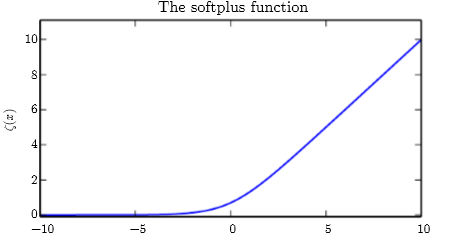
\includegraphics[width=3.5in]{fig/chap3/3_4.png}}
   \label*{图:3.5}
   \end{figure}
   \paragraph{}
   自我信息只处理一个单一的结果。我们可以使用香农熵在一个全概率分布下量化其不确定度。
   \begin{equation}
     H(x)=E_{(x\sim P)}[I(x)]=-E_{(x\sim P)}[\log{P(x)}]. \tag{3.49}
   \end{equation}
   \paragraph{}
   可以采用$H[P]$。换言之,一个分布的信息熵是来自该分布的事件的预期数量的信息。它给出了一个下界的比特数(对数以2为基础,否则单位是不同的)所需的平均编码符号服从一个分布$P$。分布几乎是确定性的(其中的结果是几乎肯定的)有低熵;有高熵的分布接近均匀。如图3.5。当$x$是连续的,其香农熵被称为微分熵。
   \paragraph{}
   如果我们有两个关于$x$的独立的概率分布$P(x)$和$Q(x)$,我们可以使用相对熵(Kullback-Leibler divergence,也称为KL散度)测量这两个分布的不同程度:
   \begin{equation}
     D_{KL}(P||Q)=E_{x\sim P}[\log{\frac{P(x)}{Q(x)}}]=E_{x\sim P}[\log{P(x)-\log{Q(x)}}].\tag{3.50}
   \end{equation}
   \paragraph*{}
   在离散型变量的情况下,它是一个额外的信息量(位测量时我们用以2为底的对数,但机器学习中我们通常使用$nats$和自然对数)需要发送一个包含来自概率分布$P$的符号的消息,我们可以使用一个准则最大限度地减少来自概率分布的消息的长度。
   \paragraph{}
   KL散度有许多有用的特性,最主要的是,它是非负的。KL散度为0表示在离散变量的情况下$p$和$q$的分布是相同的,等于一个无处不在的连续变量。因为KL散度是非负所以测量两个分布之间的差异,经常被理解为测量某种距离之间的分布。然而,它不是一个真正的距离测量,因为它不是对称的:对于$P$和$Q$,$D_{KL}(P||Q)\neq D_{KL}(Q||P)$。这种不对称性意味着对使用$D_{KL}$时选择$D_{KL}(P||Q)$ 和 $D_{KL}(Q||P)$ 哪一种对其结果影响很大。更多细节请参见图3.6。
   \paragraph{}
   和KL散度密切相关的是交叉熵,即$H (P,Q) = H(P) + D_{KL}(P||Q)$,这类似于KL散度,但如果缺少左边部分则:
   \begin{equation}
     H(P,Q)=-E_{x\sim P}\log{Q(x)}.\tag{3.51}
   \end{equation}
  \paragraph{}
  最小化相对于$Q$的交叉熵等价于最小化KL散度,因为$Q$和省略的$H(P)$不相关。
  \paragraph{}
  在计算这些量时,经常遇到0log 0这种表达形式。按照惯例,在信息论中,我们把这些表达式记为:$\lim_{x\rightarrow 0}x\log{x}=0$.
  \begin{figure}[!htb]
  \centering
   \centerline{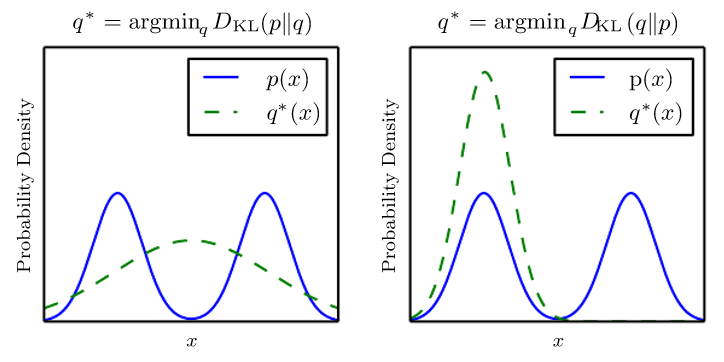
\includegraphics[width=5in]{fig/chap3/3_6.png}}
   \label*{图:3.6}
   \end{figure}
   \paragraph{}
   图3.6的KL散度是不对称的。假设我们有一个分布$P(x)$,并希望近似它与另一个分布$Q(x)$。我们要么选择最小化$D_{KL}(P ||Q)$ 或$D_{KL}(Q||P)$ 我们举例说明对$P$函数使用高斯混合计算和对$q$函数进行的高斯求解,这两种选择的不同影响。选择使用哪个方向的KL 散度是根据具体问题而言。一些应用需要一个近似,通常是高概率的任何地方,真正的分布位置的概率高,而其他应用程序需要一个近似,很少有地方高概率的真实分布的地方低概率。

    %--section 14--%

    \section*{3.14 构造概率模型}
  \paragraph{}
  在机器学习中使用概率分布通常会用到一大堆变量。通常情况下,这些概率分布只会与一部分变量直接相关。而使用一个单一的函数来描述整个联合概率分布是效率不高(无论是计算或统计方面)。
  \paragraph{}
  事实上,我们并不是使用一个单一的函数来表示一个概率分布,我们可以将一个概率分布分解成许多因素,然后相乘。例如,假设有三个随机变量:$A,B$和$C$。假设$a$影响$b$的值,$b$的影响$c$的值,但$a$和$c$相对$b$是独立的。我们可以这样来描述:
  \begin{equation}
   p(a,b,c)= p(a)p(b|a)p(c|b).\tag{3.52}
   \end{equation}
   \paragraph{}
   这样分解可以大大减少描述分布的参数。每个因数都在变量内引入了指数。这就意味着,如果我们能找到一个分解能用非常少的变量描述这个分布,那就可以大大减少描述一个分布的成本。
   \paragraph{}
   我们可以用图形来描述这些分解。这里我们用一个图形的理论,点的集合可用通过线来互联。当用图来表示因式分解的时候,我们把这个叫做结构化概率模型或图形模型。
   \paragraph{}
   有两种构造概率的模型:有方向的和无方向的。这两种图形模型使用一个图,用圆圈表示一个随机变量,一条线连接两个随机变量。用这样的方式来表示两个变量在概率分布中有直接的关系。特别的,一个有方向模型包含了分布所需的所有变量$x_{i}$,关联点的概率和它父节点的变量相关,父节点用$Pag(x_{i})$表示。
   \begin{equation}
   p(x)=\prod_{i}p(x_{i}|Pag(x_{i})).\tag{3.53}
   \end{equation}

   \paragraph{}
   无方向模型使用无方向的现将两个变量连在一块,它表示因式分解中的一系列函数。这些函数和有方向模型不同,它不是任何形式的概率分布。几个顶点连接起来叫做集合。每个集合$\mathcal{C}^{i}$在无方向模型中都会和一个因子建立关系$\phi^{(i)}(\mathcal{C}^{(i)})$,这些因子只是函数而非分布。要保证每个因子的输出都是非负的,不过不一定需要向概率分布那样,他们的和或积分为1.

   \paragraph{}
   随机变量的联合概率与所有这些因子的乘积成正比—对影响较大的因子,对其结果的影响也很大。当然,不能保证这种乘积的和一定为1。因此我们将通过除以常数$Z$进行归一化,为了获得一个归一化定义$\phi$函数产生的所有状态进行求和或积分。概率分布为:
   \begin{equation}
   p(x)=\frac{1}{Z}\prod_{i}{\o}^{(i)}(c^{(i)}) \tag{3.54}
   \end{equation}
   \begin{figure}[!htb]
   \centering
   \centerline{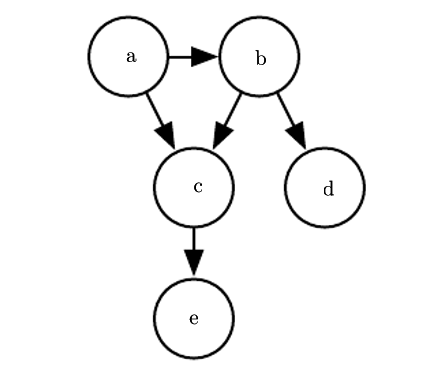
\includegraphics[width=2.5in]{fig/chap3/3_7.png}}
   \label*{图:3.7}
   \end{figure}
 \paragraph{}
 图3.7是一个有向模型的随机变量$a,b,c,d$和$e$。此图对应的概率分布可以分解为:
\begin{equation}
   p(a,b,c,d,e)=p(a)p(b|a)p(c|a,b)p(d|b)p(e|c).\tag{3.55}
 \end{equation}
\paragraph{}
 这个图可以让我们很快的看到一些分布的属性。例如,$a$和$c$之间直接影响,而$a$和$e$之间通过$c$间接影响。
 \begin{figure}[!htb]
 \centering
   \centerline{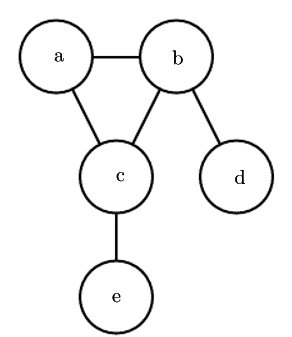
\includegraphics[width=2in]{fig/chap3/3_8.png}}
   \label*{图:3.8}
   \end{figure}
   \paragraph{}
   图3.8是一个无向模型的随机变量$a,b,c,d$和$e$。此图对应的概率分布可以分解为:
   \begin{equation}\
     p(a,b,c,d,e)=\frac{1}{Z}(a,b,c){\o}^{(2)}|(b,d){\o}^{(3)}(c,e).\tag{3.56}
   \end{equation}
   \paragraph{}
   这个图可以让我们很快的看到一些分布的属性。例如,a和c之间直接影响,而a和e之间通过c间接影响。
   \paragraph{}
   用这些图形表示分解是描述概率分布的一种语言。他们不是相互排斥的概率分布的成员。有向或无向不是一个概率分布的属性,它是一个概率分布的一个特定的描述,但任何概率分布都可以用这两种方式描述。
   \paragraph{}
   在这本书的第一部分和第二部分,我们将使用结构化的概率模型仅仅作为一种语言来描述直接概率关系和机器学习算法中的不同之处,没有进一步了解结构化的概率模型。直到讨论课题的第三部分中,我们将探索结构化概率模型中的更多细节。
   \paragraph{}
   本章回顾了深度学习相关的概率论的基本概念。其基本的数学工具仍然是:数值方法。

\end{CJK*}
\end{document}
